\section{Research Methods}

\label{s:method}

\TODO{
In this section, you would provide a description of: the research strategy (well-formulated and justified); the data collection and data analysis methods; and a clear link explaining how research strategy and methods are suitable to answer the research question(s). Include a figure providing a overview of the whole thesis in terms of research strategies/methods, RQs, inputs and outputs. An example is given in Figure}.

\lipsum[1-3]

\begin{figure*}[ht!]
    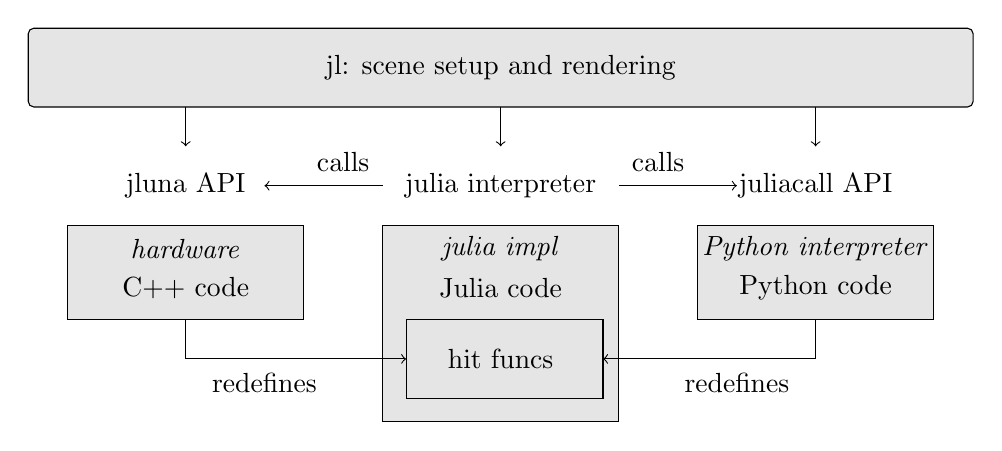
\begin{tikzpicture}
  % beveled 10x4 rectangle with text in the middle "jl: scene setup and rendering"
  \draw[rounded corners=2pt, fill=black!10] (0,0) rectangle (12,1);
  \node at (6,0.5) {jl: scene setup and rendering};
  % arrow down 2 units @ (1.5, 1)
  \draw[->] (2,0) -- (2,-.5);
  \node at (2,-1) {jluna API};
  % draw box 3 wide and 2 tall below node 
  \draw[fill=black!10] (.5,-1.5) rectangle (3.5,-2.7);
  % draw text at top of this box in italics "hardware"
  \node at (2,-1.8) {\textit{hardware}};
  \node at (2, -2.3) {C++ code};
  
  \draw[fill=black!10] (4.5,-1.5) rectangle (7.5,-4);
  \node at (6,-1.8) {\textit{julia impl}};
  \node at (6, -2.3) {Julia code};
  % draw box inside julia code box and inside that write "hit funcs"
  \draw[fill=black!10] (4.8,-2.7) rectangle (7.3,-3.7);
  \node at (6,-3.2) {hit funcs};
  
  % arrow that bends 90 degrees into julia impl from bottom of c++ box 
  \draw[->] (2,-2.7) -- (2,-3.2) -- (4.8,-3.2);
  % add text below arrow that says "redefines"
  \node at (3,-3.5) {redefines};

  % arrow down 2 units @ (7.5, 1)
  \draw[->] (10,0) -- (10,-.5);
  \node at (10,-1) {juliacall API};
  % draw box 3 wide and 2 tall below node
  \draw[fill=black!10] (8.5,-1.5) rectangle (11.5,-2.7);
  % draw text at top of this box in italics "julia impl"
  \node at (10,-1.8) {\textit{Python interpreter}};
  \node at (10, -2.3) {Python code};
  
  % arrow that bends 90 degrees into julia impl from bottom of python box
  \draw[->] (10,-2.7) -- (10,-3.2) -- (7.3,-3.2);
  % add text below arrow that says "redefines"
  \node at (9,-3.5) {redefines};

  % arrow down in the middle between above 2 
  \draw[->] (6,0) -- (6, -.5);
  \node at (6,-1) {julia interpreter};
  % arrow from julia interpreter to jluna API with the text "calls"
  \draw[->] (4.5,-1) -- (3, -1);
  \node at (4,-.7) {calls};

  % arrow from julia interpreter to juliacall API with the text "calls"
  \draw[->] (7.5,-1) -- (9, -1);
  \node at (8,-.7) {calls};
\end{tikzpicture}

    \figcap{System architecture of multi-language PBR renderer.}\label{fig:main_interface}
\end{figure*}

\lipsum[1-3]

% talk about memory optmizations 

% talk about parallelism e.g. simd, threading

% talk about compilter/interpreter optimizations 